\documentclass[letterpaper]{article} % DO NOT CHANGE THIS
\usepackage{aaai21}  % DO NOT CHANGE THIS
\usepackage{times}  % DO NOT CHANGE THIS
\usepackage{helvet} % DO NOT CHANGE THIS
\usepackage{courier}  % DO NOT CHANGE THIS
\usepackage[hyphens]{url}  % DO NOT CHANGE THIS
\usepackage{graphicx} % DO NOT CHANGE THIS
\urlstyle{rm} % DO NOT CHANGE THIS
\def\UrlFont{\rm}  % DO NOT CHANGE THIS
\usepackage{graphicx}  % DO NOT CHANGE THIS
\usepackage[numbers]{natbib}  % DO NOT CHANGE THIS AND DO NOT ADD ANY OPTIONS TO IT
\usepackage{caption} % DO NOT CHANGE THIS AND DO NOT ADD ANY OPTIONS TO IT
\frenchspacing  % DO NOT CHANGE THIS
\setlength{\pdfpagewidth}{8.5in}  % DO NOT CHANGE THIS
\setlength{\pdfpageheight}{11in}  % DO NOT CHANGE THIS
\setcounter{tocdepth}{5}
\setcounter{secnumdepth}{5}
\usepackage{amsmath}
\usepackage{hyperref}

\title{Consumer Behaviour in Retail: Next Logical Purchase using Deep Neural Network}

\author{

    %Authors
    % All authors must be in the same font size and format.
    Ankur Verma
}
\affiliations{
    %Afiliations

    %If you have multiple authors and multiple affiliations
    % use superscripts in text and roman font to identify them.
    %For example,

    % Ankur Verma, \textsuperscript{\rm 2}

    %Deep Learning Engineer \\
    % email address must be in roman text type, not monospace or sans serif
    ankur.verma.phe09@iitbhu.ac.in
}

\begin{document}

\maketitle

\begin{abstract}
% Area 
This work examines previously unseen methods of active network 
reconnaissance made possible due to the advent and popularization
of Software-Defined Networking (SDN).
% Problem
The architecture of SDN allows an adversary, controlling a compromised
switch inside the network, to perform stealthy active network
reconnaissance and gather intelligence about the network. This includes 
trying to identify sensitive resources, learn about the services, identify 
network policies, and discover potential vulnerabilities that can be exploited. 
This information can then be used in forming an attack plan to exfiltrate
sensitive data.
% Solution
We propose \name, a security application running on the controller, to
detect active reconnaissance attacks.
% Methodology
\name is implemented in Python and runs on top of a Pox controller in a
software defined network, it was tested for its ability to quickly and
accurately detect network reconnaissance in a small simulated
environment.
% Results
Our testing shows \name effectively detects network reconnaissance
with no observed false negatives or false positives and an overhead of less than 3\% on
network throughput and latency.
% Take away
This work demonstrates the need to proactivley identify new network
threats introduced by SDN before it gains a more widespread deployment.
\end{abstract}

\section{Introduction}
Consumer behaviour insights have always been one of the key business drivers for retail, specially given
fast changing consumer needs. Existing trend, competitor pricing, item reviews, sales and marketing are some of the 
key factors driving todays consumer world in retail. While very little information is available
on future variablities of the above factors, what retailers have is large volumes of transactional data.
Retailers use conventional techniques with the available data to model consumer purchase \cite{choudhury2019machine}. 
While these help in estimating purchase pattern for loyal consumers and high selling items with reasonable accuracy, they 
don't perform well for the long tail. Since multiple parameters interact non-linearly to define consumer purchase pattern,
traditional models are not sufficient to achieve high accuracy across thousands to millions of consumers.

In many of the retail/e-retail brands, short term (2-4 weeks ahead) inventory planning is done on the basis of consumer 
purchase pattern. Also, certain sales and marketing strategies like Offer Personalization, personalized item
recommendations are made leveraging results of consumer purchase predictions for the near future.
Given that every demand planner works on a narrow segment of item portfolio, there is high 
variability in choices that different planners recommend. Also, given their busy schedule, they have very less interaction
moments to discuss their views and insights over their recommendations. Hence, subtle effects like cannibalization
\cite{shah2007retailer}, and item-affinity remains unaccounted. Such inefficiencies lead to gap between consumer needs 
and item availablity, resulting in the loss of business opportunities in terms of consumer churn, out-of-stock, 
and excess inventory.

In this paper, we apply multiple deep learning architectures along with tree based machine learning algorithms
to predict the next logical item purchase at consumer level. We showcase the performance of individual models with 
varying hyper-parameter configurations along with the results of stacked generalization ensemble \cite{wolpert1992stacked} 
(algorithmic combination of predictions from different models) and F\textsubscript{1}-maximization (optimal purchase 
probability cut-off at consumer level).
In the next section \ref{sec:relatedwork}, we briefly discuss research work related to the problem in hand. 
Section \ref{sec:methodology} explains the overall methodology adopted to solve the problem.
It lays out and neural network architectures and various algorithmic variants applied to the problem.
Section \ref{sec:eval} describes the experiments performed, and results obtained in different modelling setups.

\section{Related Work}
\label{sec:relatedwork}
In the past few years, usefullness of various machine learning methods for predicting consumer purchase pattern have been 
analyzed in the academia field and few of them are often used by ML practitioners. In most cases many of those approaches are 
based on extracting consumer's latent characteristics from its past purchase behavior and applying statistical and  
ML based formulations \cite{fader2009probability, choudhury2019machine}. 
Some previous studies have analyzed the use of random forest and Xgboost techniques in order to predict 
consumer retention, where past consumer behavior was used as potential explanatory variable 
for modelling such patterns. In one such study \cite{martinez2020machine}, the authors develop a model for predicting whether a 
consumer performs a purchase in prescribed future time frame based on historical purchase information such as the number
of transactions, time of the last transaction, and the relative change in total spending of a consumer. 
They found gradient boosting to perform best over test data. We propose neural network architectures with entity embeddings
\cite{guo2016entity} which outperform the gradient boosting type of models like Xgboost \cite{chen2016xgboost}. 

From Neural Network architectures perspective,
close to our work is Deep Neural Network Ensembles for Time Series Classification \cite{fawaz2019deep}. 
In this paper, authors show how an ensemble of multiple Convolutional Neural Networks can improve upon the 
state-of-the-art performance of individual neural networks. They use 6 deep learning classifiers 
including Multi Layer Perceptron, Fully Convolutional Neural Network, Residual Network, 
Encoder \cite{serra2018towards}, Multi-Channels Deep Convolutional Neural Networks \cite{zheng2014time} and 
Time Convolutional Neural Network \cite{zhao2017convolutional}. The first three were originally proposed in \cite{wang2017time}.
We propose the application of such architectures in the consumer choice world and apply the concept of entity embeddings 
\cite{guo2016entity} along with neural network architectures
like Multi Layer Perceptron, Long Short Term Memory (LSTM), Temporal Convolutional Networks (TCN) \cite{lea2016temporal} and 
TCN-LSTM \cite{karim2017lstm}.

\section{Methodology}
\label{sec:methodology}

\begin{figure}[h]
\begin{center}
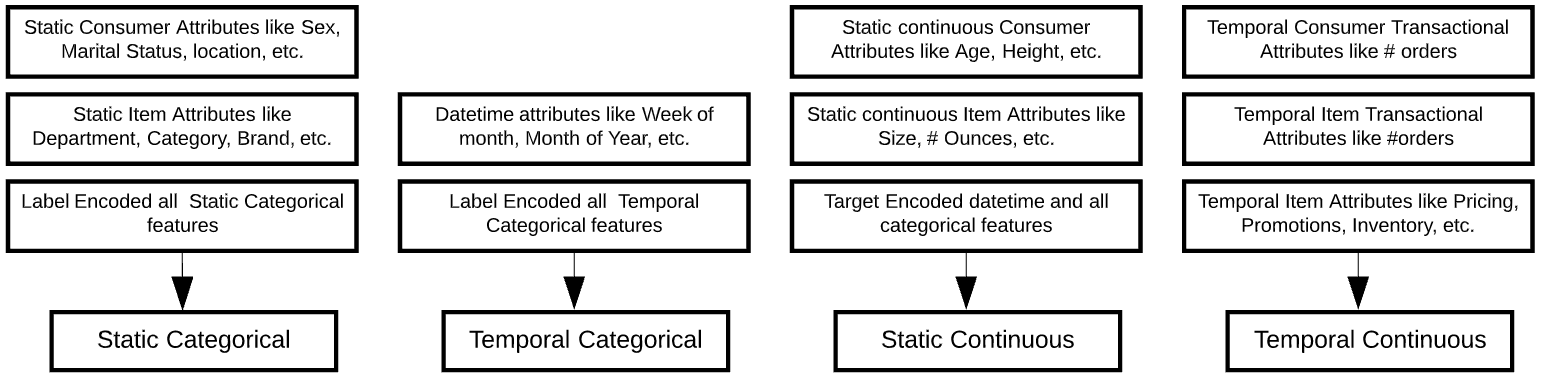
\includegraphics[width=4.4in]{img/dnndata.png}
\end{center}
\caption{Data classification for DNN Architectures}
\end{figure}

\begin{figure}[h]
\begin{center}
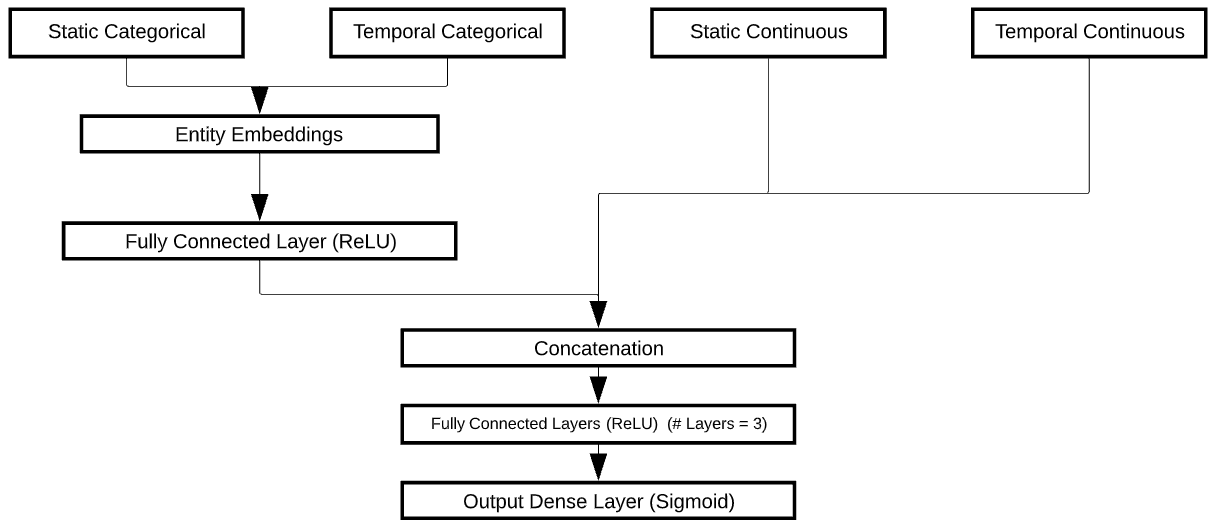
\includegraphics[width=4.4in]{img/MLP.png} 
\end{center}
\caption{Multi Layer Perceptron Architecture}
\end{figure}

\section{Experiments and Results}
\label{sec:eval}

\subsection{Loss Function}
The models have been judged on various criteria for their Mean Absolute Percent Error.
As discussed in section III(B), 13 weeks of data for each UPC has been kept as test data. We calculate MAPE for each of
these UPCs by doing prediction on test data using the trained model. It is an indicator of how accurate the models are. 
A model has been considered a legitimate model only if the MAPE is less than 30%.

\subsection{Model Stability} 
The products available in Walmart have dynamic nature, their nature and characteristics keep on changing over time. 
In this regard, it becomes very important to ensure that models which have been built are robust and successfully 
capture the dynamic nature of the products. 

To do this, a model for an UPC has been trained on datasets having same features but are of different time periods. 
This has been done on five different datasets for an UPC and elasticity values have been generated using the simulation 
technique as described in section II(C). The average change in coefficient values of price variables as well as elasticity 
values for all the UPCs was less than 10% across all of these time periods. This test makes sure that the model is not 
getting overfit on the train data. 

\subsection{Volume Lift Accuracy}  
As discussed in previous sections, most of the products in the Walmart eco-system do not go through significant 
number of price changes, in order to estimate the performance of the models during a price change, volume lift 
accuracy has been calculated. 

This has been done by considering all those weeks where     
price change has occurred in train and test data. In all those weeks, next eight weeks of actual 
as well as predicted volume have been taken and MAPE, discussed above, has been calculated. The rationale behind
taking next eight weeks is that the effect of a price change such as jump in demand has always been observed at 
least a week after the price change. One of the reasons behind this lag is customers take time to internalize the price 
change and react to it.

\subsection{Discussion}  
Walmart landscape. 

Table III discusses the overall coverage of our models for 40 odd categories available in Walmart eco-system. 
To get coverage of a model, we only consider UPCs which have models with MAPE less than 30%. In addition to this, 
only the UPCs which have elasticity in range [-4,0) have been considered. The baseline for the coverage calculation 
includes only those items which have been sold in more than 2000 stores in last 1 year to include only national items not 
regional items. 

Total number of UPCs column in Table III gives the baseline for the categories and other columns depict the coverage 
from three different models. The last column is the overall coverage which has been found by combining the results of 
three different models.

Consider the category number 1867 in Table III, this category has 729 UPCs which have been sold in more than 2000 stores 
in 1 year, out of which ,561 UPCs have been successfully captured by these three models i.e. 561 UPCs are more than 70% 
accurate and have elasticity in [-4,0). Similarly, category 1483 has exceptionally good coverage of 97%. However, coverage 
is not satisfactory for all the categories for e.g., category 8539(Television) has overall coverage quite low. One of the 
reasons might be highly elastic nature of electronic appliances. This shows that other approaches also need to be tried out
 to capture these nuances. 

Table IV summarizes the coverage from three models. Overall, the line, fineline and category models are capturing 70% 
of national items for these 40 odd categories. 


\section{Conclusion}
We have presented the study of the Consumer behaviour with Deep Neural Networks and shown how
DNNs outperform the Machine Learning models like Xgboost and RandomForest. We also showcase the 
potential of stacked generalisation as well as F1-Maximization.


%\clearpage
\bibliography{paper}
\end{document}
